\section{Direct Manipulation Language for Explaining Algorithms}

CodeInk includes a visual vocabulary for common data structures and a direct
manipulation language for describing primitive behaviors that occur in commonly
taught algorithms. In this section, we describe the scope of this work, and
present our visual vocabulary and direct manipulation language.

\subsection{Scope: concrete traces and visual problems}

We scoped our language design in two ways to suit its role in educational
scenarios. First, we focus on demonstrations of an algorithm's trace on a
concrete example rather than its behavior on any arbitrary input. Instructors
often first explain an algorithm by diagramming its behavior on a specific
example rather than by writing pseudocode on the board and illustrating its
general behavior on some abstract representation. Our language focuses on this
common scenario, allowing the user to set up an example data structure and trace
the algorithm by directly manipulating data on the canvas.

Second, our language focuses on supporting algorithm traces for lists, binary
trees, and graphs, because their canonical algorithms -- sorting, rotation,
search and shortest paths -- are widely taught in introductory CS and algorithms
classes. These data structures and their associated algorithms are also
inherently visual: The natural way to teach and think through them is by drawing
diagrams. Thus, we envision direct manipulation languages for describing
computation to be most useful for these types of problems.
%
%Also, they represent around \todo{50\%} of the algorithms covered in
%CLRS~\cite{Cormen2001}, one of the most popular algorithms textbooks. 
%
In \sec{sec:design-and-future-work}, we discuss how our language can be
extended to support demonstrations of an algorithm's general behavior
across more kinds of data structures.

\begin{figure} %[!b]

\begin{center}
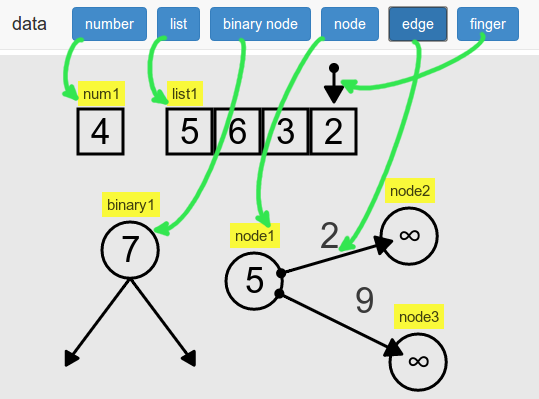
\includegraphics[width=0.8\columnwidth]{img/visual-vocabulary.png}
\end{center}

\vspace{-0.75em}
\caption{CodeInk's visual vocabulary. The green arrows (for illustration only)
show how numbers, lists, binary tree nodes, graph nodes, edges and fingers are
visually represented in CodeInk.}

\label{fig:visual_vocab}
\end{figure}

\subsection{CodeInk's visual vocabulary}

CodeInk's visual vocabulary (\fig{fig:visual_vocab}) is modeled after our
observations of instructors explaining data structures and algorithms in MIT's
introductory programming and algorithms courses. For example, in those courses a
binary tree node is represented visually as a circle with a number as its key
value and two arrows as its left and right pointers; CodeInk mirrors this visual
representation. The vocabulary currently supports numeric
values, which is sufficient for many algorithms. We plan to add support for
strings in the future.

We have also implemented a special construct called a \emph{finger}, which
points to any on-screen visual object. This can express the current point in a
traversal algorithm, like a \emph{curr} pointer. In an educational setting, the
finger replaces the instructor pointing to a particular object during lecture.

\subsection{CodeInk's direct manipulation language}

Our direct manipulation language enables users to perform gestures on live data
structures to trace an algorithm's behavior. Almost every user interaction
has some programmatic interpretation in Python.
% In contrast, when drawing and redrawing diagrams on blackboards or PowerPoint,
% objects either cannot be manipulated, or can be dragged around but without any
% programmatic interpretation.
To design this language, we watched lectures from MIT's
introductory CS and algorithms courses that featured worked examples of
lists, trees, and graphs. We asked three questions:

\begin{itemize}

  \item What behaviors need to be expressed to explain each algorithm's
  trace on the example data structure?

  \item How do instructors currently express those behaviors by drawing
  on the blackboard?

  \item What direct manipulation gestures would be most natural to
  express those behaviors?

\end{itemize}

We devised a compact set of eight gestures (\tab{tbl:language_table})
that cover common algorithms on lists, trees, and graphs.

%We now explain the gestures by demonstrating how a user would explain
%insertion sort on a list, an AVL insertion on a binary tree, and
%Dijkstra's algorithm on a graph.


\begin{figure}

\begin{center}
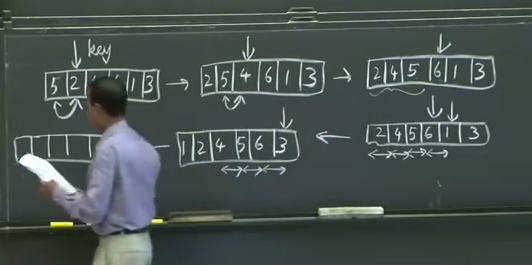
\includegraphics[width=0.7\columnwidth]{img/6006/insertion.png}
\end{center}

\vspace{-0.75em}
\caption{An instructor of MIT's introductory algorithms class draws
blackboard diagrams to explain insertion sort on an example of a list.}
\vspace{-0.75em}
\label{fig:6006-insertion}
\end{figure}


\noindent \textbf{List algorithms}:
List sorting and searching are fundamental topics in algorithms courses. Describing insertion
sort, for instance, requires the user to express the following behaviors:
creating a list, maintaining a pointer to the current list position, comparing
numeric values, and swapping elements. Instructors typically describe these
behaviors on the blackboard by redrawing the list in new configurations, with
arrows showing transitions between states (\fig{fig:6006-insertion}).
Here is how to demonstrate insertion sort in CodeInk:

\noindent 1) Drag an example list onto the canvas and type in a list of numbers
to initialize its values. Indicate the current list position by dropping a
finger onto the second element (green arrows indicate drag motion and
are not part of the CodeInk UI).

\vspace{-0.25em}
\noindent 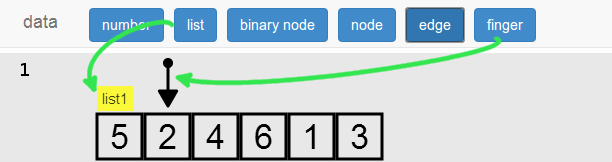
\includegraphics[width=0.7\columnwidth]{img/examples/insertion-1.png}
\vspace{0.5em}

\noindent 2) To prepare to move the ``2" element, grab and hold the element for
at least one second (\emph{dwell}). A blue circle fills up to give the user
feedback on how long they have dwelled.

\vspace{-0.25em}
\noindent 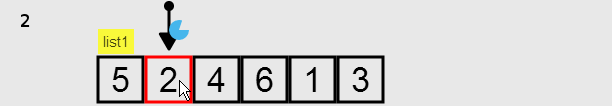
\includegraphics[width=0.7\columnwidth]{img/examples/insertion-2.png}
\vspace{0.4em}

\noindent 3) After one second has elapsed (blue circle filled entirely), the
list expands outward, creating gaps into which the dragged element can be
inserted. The ``2" element is ready to be moved.

\vspace{-0.25em}
\noindent 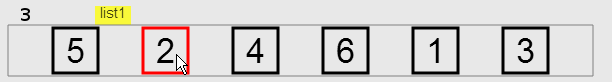
\includegraphics[width=0.7\columnwidth]{img/examples/insertion-3.png}
\vspace{0.5em}

\noindent 4) Drag the ``2" to the left until it hits the ``5" element, which
creates a numeric comparison step (``2 $<$ 5") in the trace.

\vspace{-0.25em}
\noindent 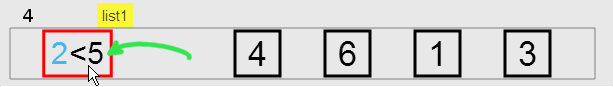
\includegraphics[width=0.7\columnwidth]{img/examples/insertion-4.png}
\vspace{0.5em}

\noindent 5) Keep moving the ``2" to the left of the ``5" element.

\vspace{-0.25em}
\noindent 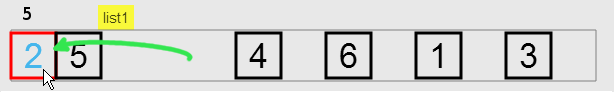
\includegraphics[width=0.7\columnwidth]{img/examples/insertion-5.png}
\vspace{0.5em}

\noindent 6) Once the correct position is found, drop the element
to create a list insertion step in the trace. The list collapses again in its new, rearranged state, with the
``2" preceeding the ``5''.

\noindent 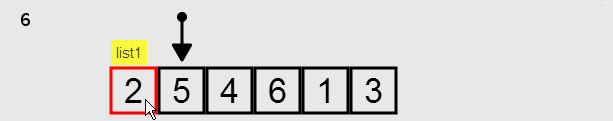
\includegraphics[width=0.7\columnwidth]{img/examples/insertion-6.png}

The user explains the rest of insertion sort by moving the finger down the list
and inserting the current element into the sorted sublist until the entire list
is sorted. If any mistakes are made, the user can undo steps to remove them
from the trace. The steps can be played back and also shared online.
Many list sorting and searching algorithms can be explained using this subset of CodeInk's direct
manipulation language: creating lists, using fingers to indicate traversal
points, and dragging list elements to show comparisons and rearrangements.


%\begin{figure}[!h]
%\caption{An instructor in MIT's introductory algorithms class explains
%the insertion of several values into an AVL.}
%\label{fig:6006-bst}
%\end{figure}

\begin{figure}

\begin{center}
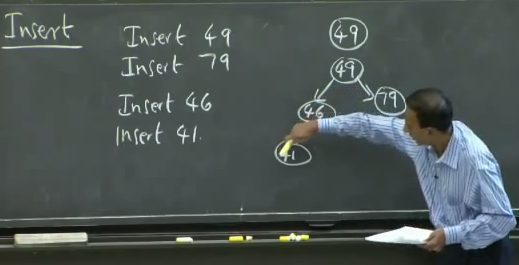
\includegraphics[width=0.7\columnwidth]{img/6006/bst.png}
\end{center}

\vspace{-0.75em}

\caption{An instructor demonstrating AVL (balanced binary search) tree
inserts.}
\vspace{-0.75em}

\label{fig:example-bst}
\end{figure}


\noindent \textbf{Binary tree algorithms}:
Common tree algorithms, such as an AVL (balanced binary search tree) insertion,
require creating binary tree nodes, comparing node values, recursing into a
node's left or right child, inserting nodes, and rotating subtrees. Instructors
sometimes visualize a tree traversal pattern by drawing a line along the
appropriate pointer and zig-zagging down the tree (see \fig{fig:example-bst}). They illustrate tree rotations by completely redrawing
the tree in a new configuration, which is tedious and error-prone. Here is how
to trace a series of AVL tree insertions in CodeInk:

\noindent \begin{tabular}{m{4.6cm} m{3.4cm}}

1) Create two new binary tree nodes (``4" and ``6") by dragging node
objects onto the canvas and typing in their values.

& 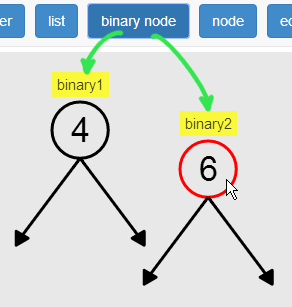
\includegraphics[width=3.4cm]{img/examples/bst-1.png}
\end{tabular}


\noindent \begin{tabular}{m{4.6cm} m{3.4cm}}

2) Drag the ``6'' node into the ``4'' node to compare their values.
CodeInk adds the comparison step (``4 $<$ 6") to the trace.

& 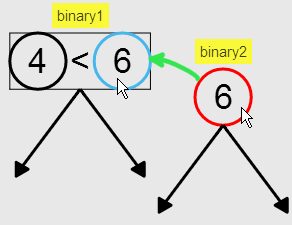
\includegraphics[width=3.4cm]{img/examples/bst-2.png}
\end{tabular}

\noindent \begin{tabular}{m{6.2cm} m{1.8cm}}

3) Since ``6" is greater than ``4", keep dragging the ``6'' along the
right pointer of the ``4" node. This temporarily highlights the pointer
blue and adds a \emph{pointer traversal} step to the trace.

& 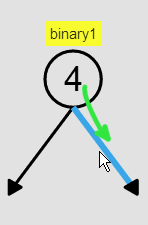
\includegraphics[width=1.8cm]{img/examples/bst-3.png}
\end{tabular}

\noindent \begin{tabular}{m{4.6cm} m{3.4cm}}

4) Keep dragging along the right pointer until reaching its tip. The
``6" node now re-emerges as the right child of ``4." The node is colored blue to
preview the insertion. Release the node to confirm the insertion:
\texttt{binary1.right = binary2}

& 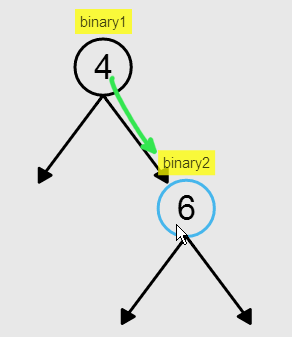
\includegraphics[width=3.4cm]{img/examples/bst-4.png}
\end{tabular}

\noindent \begin{tabular}{m{4.6cm} m{3.4cm}}

5) Next insert a new ``9" node into the tree, which results in an
unbalanced tree. Now demonstrate a rotation by grabbing the ``6" node,
dwelling for one second, and dragging it away to detach the subtree.
When the subtree is dropped on the canvas, a new step is added to the
trace: \texttt{binary1.right = None}

& 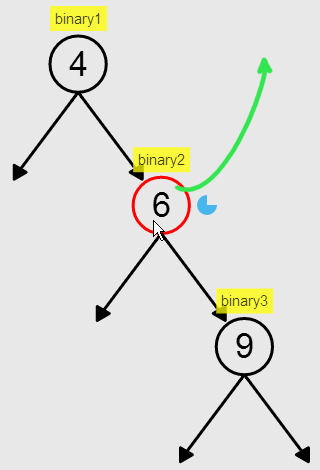
\includegraphics[width=3.4cm]{img/examples/bst-5.png}
\end{tabular}

\noindent \begin{tabular}{m{4.6cm} m{3.4cm}}

6) The ``6 / 9" subtree is now separated from the ``4." Drag the ``4"
node downward ...

& 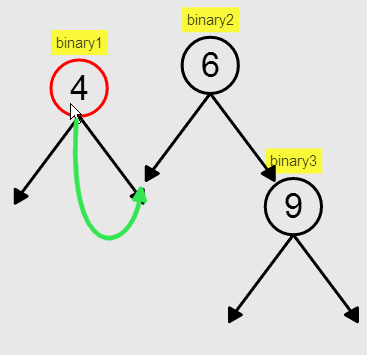
\includegraphics[width=3.4cm]{img/examples/bst-6.png}
\end{tabular}

\noindent \begin{tabular}{m{4.6cm} m{3.4cm}}

7) ... until it reaches the tip of the ``6" node's left pointer, then
release to insert it there and balance the tree: \texttt{binary2.left =
binary1}

& 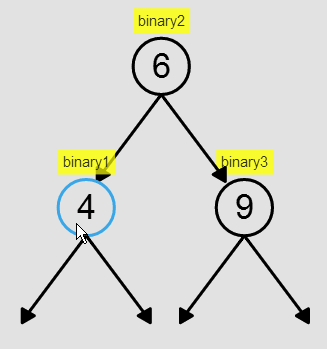
\includegraphics[width=3.4cm]{img/examples/bst-7.png}
\end{tabular}

As is the case with lists, dragging one value into another triggers a
numeric comparison (step 2), and grabbing and dwelling on a child object
removes it from its parent data structure (step 5).

\begin{figure}
\begin{center}
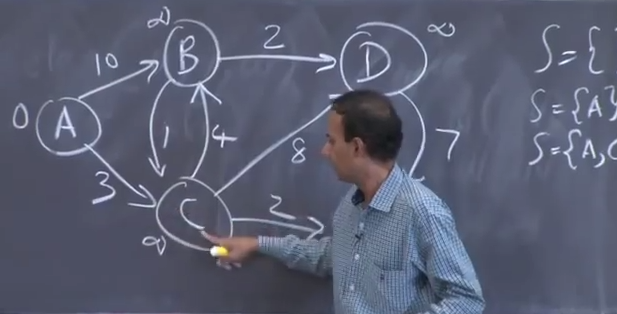
\includegraphics[width=0.7\columnwidth]{img/6006/dijkstra.png}
\end{center}

\vspace{-0.75em}

\caption{An instructor demonstrating Dijkstra's algorithm on the
blackboard.}
\vspace{-0.75em}

\label{fig:example-dijkstra}
\end{figure}


\noindent \textbf{Graph algorithms}: Our language also covers graph
traversal, such as search or finding shortest paths (see
\fig{fig:example-dijkstra}). It supports creating and attaching graph
nodes and edges, updating node and edge values, and marking nodes as
visited. Here is how to trace Dijkstra's algorithm using CodeInk:

\noindent \begin{tabular}{m{4.2cm} m{3.8cm}}
1) Create an example graph by dragging and dropping node and edge
objects onto the canvas, typing in the numeric node costs and edge weights.
Edges can be connected to nodes by clicking and dragging their start and end
handles.
& 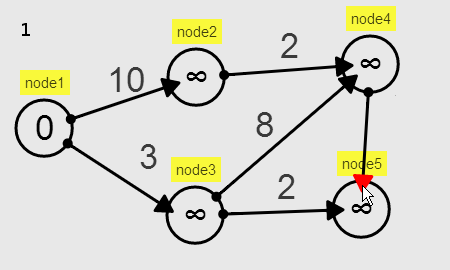
\includegraphics[width=3.8cm]{img/examples/dijkstra-1.png}
\end{tabular}

\noindent \begin{tabular}{m{4.2cm} m{3.8cm}}
2) Start with \texttt{node1}. To calculate the
cost of reaching its neighbor \texttt{node2},
first drag \texttt{node1} (source node) and drop it onto the canvas, which
creates a new number (\texttt{num1}) equal to the node's cost (\texttt{0}).
& 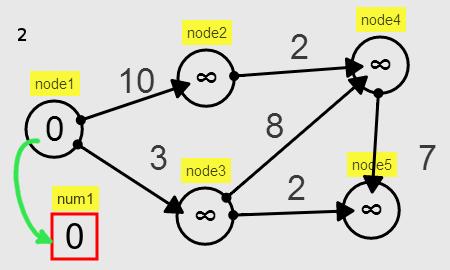
\includegraphics[width=3.8cm]{img/examples/dijkstra-2.png}
\end{tabular}

\noindent \begin{tabular}{m{4.2cm} m{3.8cm}}
3) Now drag the weight of the connecting edge into the current cost
(\texttt{num1}), which triggers a comparison by default. However, a
comparison is not the correct operation; the two values
must be added.
& 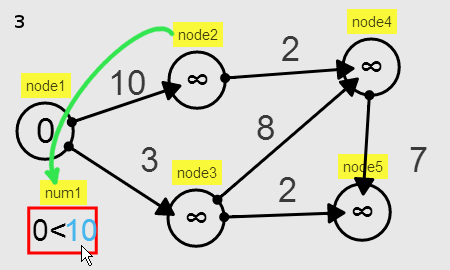
\includegraphics[width=3.8cm]{img/examples/dijkstra-3.png}
\end{tabular}

\noindent \begin{tabular}{m{4.2cm} m{3.8cm}}
4) Dwelling after the drag-into gesture causes CodeInk to cycle through alternative
interpretations. When an addition assignment
operation (\texttt{+=}) appears, release to end the gesture. The cost
updates to the value of \texttt{10} (\texttt{num1 += edge1.weight}).
& 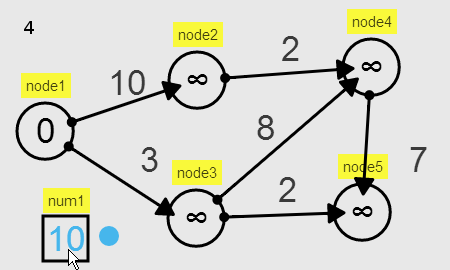
\includegraphics[width=3.8cm]{img/examples/dijkstra-4.png}
\end{tabular}

\noindent \begin{tabular}{m{4.2cm} m{3.8cm}}
5) Now drag \texttt{num1} into \texttt{node2}
to trigger a comparison, checking if the new cost is less than
the existing cost of reaching that node.
& 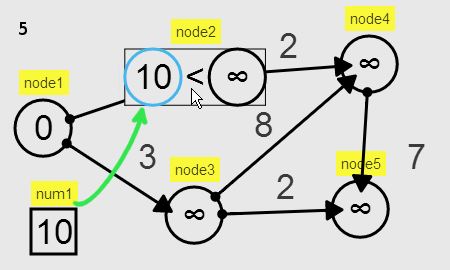
\includegraphics[width=3.8cm]{img/examples/dijkstra-5.png}
\end{tabular}

\noindent \begin{tabular}{m{4.2cm} m{3.8cm}}
6) Since \texttt{10 $<$ $\infty$}, dwell to cycle to the assignment
expression (\texttt{node2.value = num1}). Releasing ends the gesture, and updates the cost
of \texttt{node2} to 10.
& 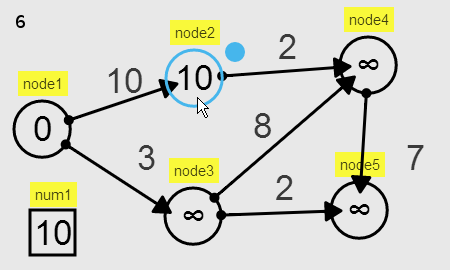
\includegraphics[width=3.8cm]{img/examples/dijkstra-6.png}
\end{tabular}

\noindent \begin{tabular}{m{4.2cm} m{3.8cm}}
7) Repeat on all nodes and mark each one as visited by
selecting ``Fill" and clicking on that node.
& 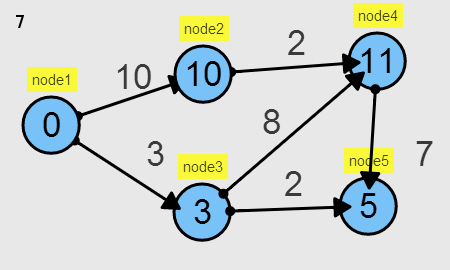
\includegraphics[width=3.8cm]{img/examples/dijkstra-7.png}
\end{tabular}

%Because the drag-into gesture has multiple interpretations
%(comparison, assignment, addition assignment), the user can dwell
%to cycle through all interpretations (see \sec{sec:overloaded-gestures}).

\noindent \textbf{Unified DM language}:
Table \ref{tbl:language_table} summarizes CodeInk's direct manipulation language.
While the preceding examples appear different, our
language's gesture set generalizes across the primitive behaviors in each
algorithm. For example, the user can copy a numeric value using the drag-away
gesture, regardless of whether the value is a list element or tree/graph node.
Similarly, comparing two values is always explained by the drag-into gesture,
regardless of whether the values are both node values, list elements or some
heterogeneous pair. This expressivity means the language can be used to describe
a variety of list, tree and graph algorithms (see
\sec{sec:design-and-future-work}).

We turn next to two subtle language design decisions: chaining of gestures and
resolving overloaded gestures.

\begin{table}[!t]
\vspace{-2em}
% % increase table row spacing, adjust to taste
\renewcommand{\arraystretch}{1.75}
% if using array.sty, it might be a good idea to tweak the value of
% \extrarowheight as needed to properly center the text within the cells
% \setlength{\extrarowheight}{10pt}
\caption{CodeInk's Direct Manipulation Language}
\label{tbl:language_table}
\centering
% % Some packages, such as MDW tools, offer better commands for making tables %
% than the plain LaTeX2e tabular which is used here.
\begin{tabular}{|p{3.8cm} |p{3.8cm} |}
\hline
\textbf{Program Behavior} & \textbf{DM Gesture} \\
\hline
%Access a value & Grab value and drag elsewhere \\
%\hline
Copy a value & {\em drag-away}: Grab an object, and drag it away quickly.
Drop it on the canvas to create a new number with the same value.
\\
\hline
Remove a list element, or detach a tree/graph node from its parents &
{\em dwell-drag-away}: Grab an object, dwell for one second, then
drag it elsewhere.
\\
\hline
Compare two values & {\em drag-into}: Drag one value into another.
\\
\hline
Assign one object's value to another &
{\em drag-into-dwell}: Drag one value into another, and
dwell until the desired interpretation (\texttt{=, +=, -=}) appears. \\
\hline
Insert a value into a list, or a node into a tree/graph
& {\em drag-insert}: Drag the value into a gap in the list, or the node to the
tip of an edge
\\

\hline
Attach an edge to a graph node
& {\em drag-edge}: Drag the edge's start or end handle to the node.
\\

\hline
Mark a list element or tree/graph node (e.g. as sorted or visited) &
{\em fill}: Select the ``Fill" tool, and click on the element. \\
\hline
Indicate the current traversal point & {\em drag-finger}: Drag the finger to a
list element or tree/graph node.
\\
\hline
\end{tabular}
\end{table}

\subsection{Chaining and traversal patterns}
The user can chain multiple gestures while dragging an object. One common
example of chaining arises when describing a traversal pattern involving a
series of comparisons. For example, during insertion sort, the user can drag an
element along the list, performing comparisons without releasing it until the
correct location is found. When the location is found, the user can release the
element into the gap between two existing elements, resulting in an insertion.

One subtle interaction issue during a chain of gestures is deciding which
behaviors to commit to the list of steps, and which to omit. For example, the
user should be allowed to drag an element into a list, then undo the behavior by
dragging it back out of the list. The insertion should be committed only when
the new value is released into the list. However, other behaviors like
comparisons should be committed while the user continues to drag, since they are
performed as part of the traversal pattern. Note that in the insertion sort
demonstration, there is only one grab, drag, and release, but both the
numeric comparison and swap are added to the trace. The same applies for
the AVL insertion, where the candidate node is dragged
through the tree in one motion, until it is released at a leaf.

In exploring this issue of which behaviors to commit, we have found it useful to
distinguish between mutation and observation behaviors. Mutation behaviors are
those that result in data structure changes (e.g., insertions, assignments), while
observation behaviors only visualize decision making in the algorithm
(e.g., comparisons, following pointers), and do not affect the underlying data
structures. In a chain of gestures, observation behaviors are continuously
committed to the algorithm's trace, while mutation behaviors are committed
only if the data structure has changed at the end of a gesture.

\subsection{Resolving overloaded gestures}
\label{sec:overloaded-gestures}

When designing a gesture vocabulary, the gesture that seems most natural for a
task can often be interpreted in multiple ways. There are two main examples of
this in CodeInk's language: ambiguity in the drag-into gesture, and ambiguity in
the drag-away gesture when the value is part of some higher-level data structure
(e.g. a list element, or a child node in a tree or graph).

The drag-into gesture is ambiguous because dragging one object into
another could be interpreted as a comparison (\texttt{x$<$y}), an
assignment (\texttt{x=y}), or an augmented assignment such as
\texttt{x+=y} or \texttt{x-=y}.

Performing the drag-away gesture on a child object is ambiguous because it is
not obvious whether the parent object should be altered or not. For example,
when dragging an element away from a list, should a copy of the element be made,
or should the element be pulled out of the parent list? For trees and graphs,
should a copy of the dragged node be made, or should that node and its
descendants be detached from the parent?

Our solution is to default to the observation behavior of a gesture, and preview
other possible mutation behaviors if the user dwells for more than one second.
This means defaulting to a comparison for the drag-into gesture, and making a
copy of the dragged value for the drag-away gesture.
%
This is also useful for a chained traversal pattern, since the comparisons
can occur in quick succession while dragging without dwelling.

%In order to make an assignment, the user can drag the source object into
%the target and dwell. At that point, the system cycles through different
%interpretations of the gesture. In the case of dragging a child object,
%the user selects and dwells on a list element or node until it turns
%blue, indicating it has been detached from its parent.
